\documentclass[tikz,border=10pt]{standalone}
\usetikzlibrary{arrows,positioning,shadows}

\begin{document}
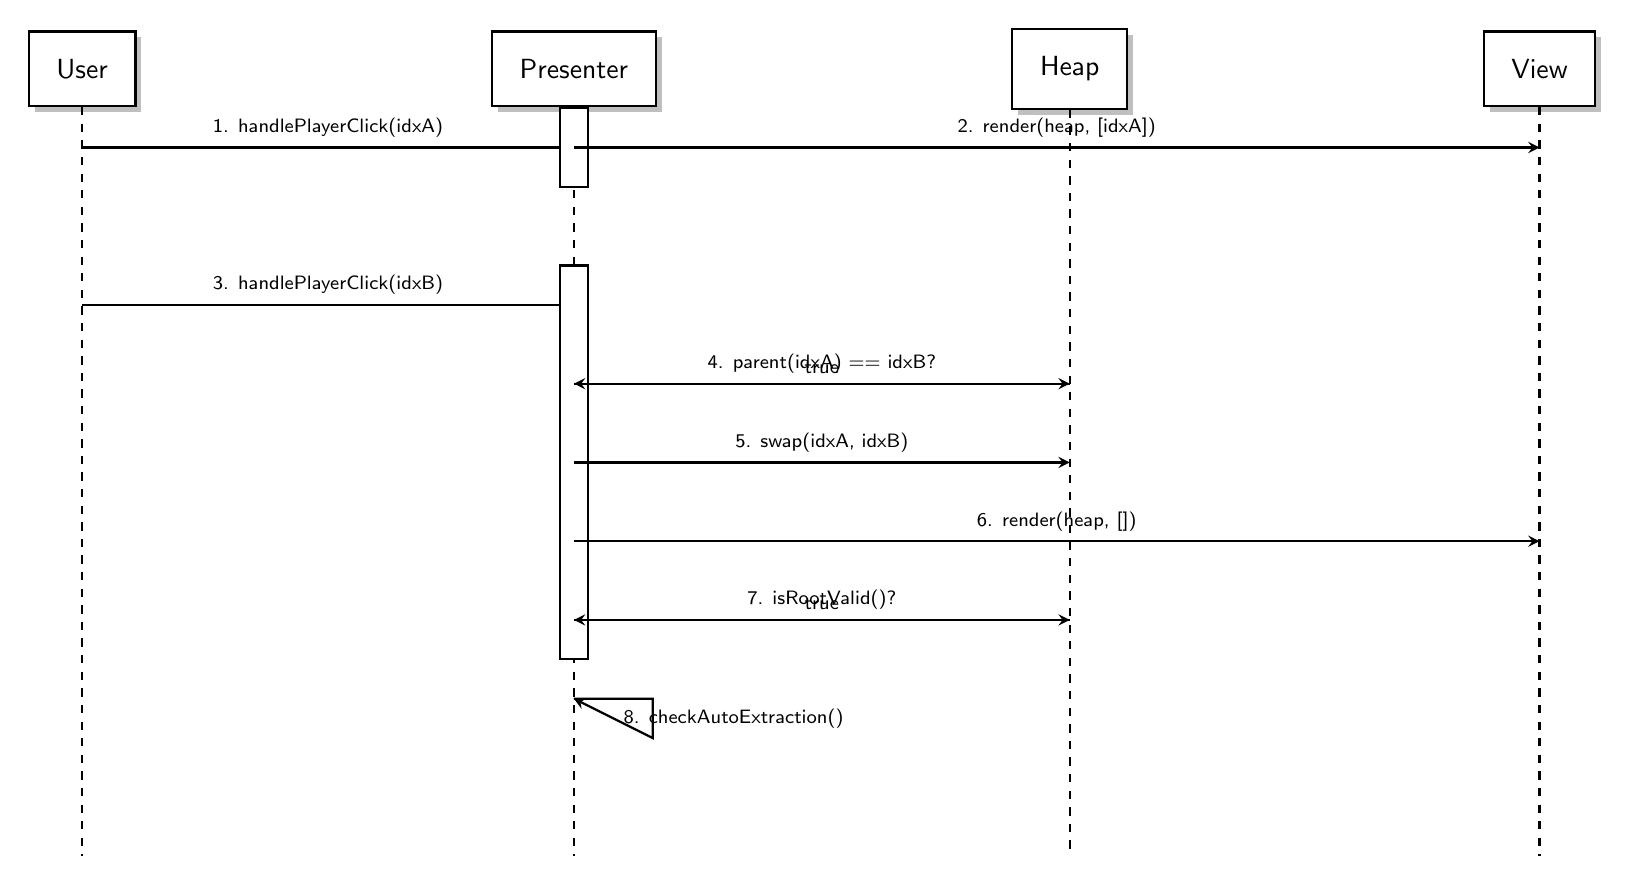
\begin{tikzpicture}[font=\sffamily, thick,
    actor/.style={draw, fill=white, inner sep=10pt, drop shadow},
    lifeline/.style={draw, dashed},
    activation/.style={draw, fill=white, minimum width=10pt},
    mess/.style={->, >=stealth}
]

% Actors (Increased spacing to 4.5cm for better readability)
\node[actor] (User) {User};
\node[actor, right=4.5cm of User] (Presenter) {Presenter};
\node[actor, right=4.5cm of Presenter] (Heap) {Heap};
\node[actor, right=4.5cm of Heap] (View) {View};

% Lifelines
\draw[lifeline] (User) -- ++(0,-10) coordinate (UserBottom);
\draw[lifeline] (Presenter) -- ++(0,-10) coordinate (PresenterBottom);
\draw[lifeline] (Heap) -- ++(0,-10) coordinate (HeapBottom);
\draw[lifeline] (View) -- ++(0,-10) coordinate (ViewBottom);

% Time steps coordinates (roughly)
\coordinate (t1) at (0,-1);
\coordinate (t2) at (0,-2);
\coordinate (t3) at (0,-3);
\coordinate (t4) at (0,-4);
\coordinate (t5) at (0,-5);
\coordinate (t6) at (0,-6);
\coordinate (t7) at (0,-7);
\coordinate (t8) at (0,-8);
\coordinate (t9) at (0,-9);

% 1. Click Node A
\draw[mess] (User |- t1) -- node[above,midway] {\scriptsize 1. handlePlayerClick(idxA)} (Presenter |- t1);
\node[activation, minimum height=1cm] at (Presenter |- t1) {};

% 2. Render Selection
\draw[mess] (Presenter |- t1.south) -- node[above,midway] {\scriptsize 2. render(heap, [idxA])} (View |- t1.south);
% \node[activation, minimum height=0.5cm] at (View |- t1.south) {};

% 3. Click Node B
\draw[mess] (User |- t3) -- node[above,midway] {\scriptsize 3. handlePlayerClick(idxB)} (Presenter |- t3);
\node[activation, minimum height=5cm] (PresAct) at (Presenter |- t5.5) {}; % Long activation

% 4. Check Validity
\draw[mess] (Presenter |- t4) -- node[above,midway] {\scriptsize 4. parent(idxA) == idxB?} (Heap |- t4);
\draw[mess, dashed] (Heap |- t4.south) -- node[above,midway] {\scriptsize true} (Presenter |- t4.south);

% 5. Swap
\draw[mess] (Presenter |- t5) -- node[above,midway] {\scriptsize 5. swap(idxA, idxB)} (Heap |- t5);

% 6. Render new state
\draw[mess] (Presenter |- t6) -- node[above,midway] {\scriptsize 6. render(heap, [])} (View |- t6);

% 7. Check Root
\draw[mess] (Presenter |- t7) -- node[above,midway] {\scriptsize 7. isRootValid()?} (Heap |- t7);
\draw[mess, dashed] (Heap |- t7.south) -- node[above,midway] {\scriptsize true} (Presenter |- t7.south);

% 8. Auto Extraction
\draw[mess] (Presenter |- t8) -- ++(1,0) -- ++(0,-0.5) -- node[right,midway] {\scriptsize 8. checkAutoExtraction()} (Presenter |- t8.south);

\end{tikzpicture}
\end{document}
